\section*{Problem 4 - Attitude Control using Rotation matrices}

 
\subsection*{Problem 4.1}
\begin{equation}
    \boldsymbol{\tau}=-\boldsymbol{K}_d\boldsymbol{\omega} - \boldsymbol{K}_p\boldsymbol{\Omega}_a(\boldsymbol{R})
\end{equation}
\begin{equation}
\boldsymbol{\Omega}_{\boldsymbol{a}}(\boldsymbol{R}) := \sum \limits_{i=1}^3 a_i \boldsymbol{e}_i \times (\boldsymbol{R}_d^{\top} \boldsymbol{R} \boldsymbol{e}_i)
\end{equation} 

Since $\boldsymbol{R_d}$ is orthogonal, $\boldsymbol{R_d}^T\boldsymbol{R_d}=\boldsymbol{I}$
\begin{subequation}
\begin{align}
\boldsymbol{\Omega}_{\boldsymbol{a}}(\boldsymbol{R}_d) &=  \sum \limits_{i=1}^3 a_i \boldsymbol{e}_i \times (\boldsymbol{I} \boldsymbol{e}_i)\\
&= \sum \limits_{i=1}^3 a_i \boldsymbol{e}_i \times \boldsymbol{e}_i
= \sum \limits_{i=1}^3 a_i\boldsymbol{0}
= \boldsymbol{0}
\end{align}
\end{subequation}
\subsection*{Problem 4.2}
The attitude error is $\boldsymbol{\tilde{R}}=\boldsymbol{R}_d^T\boldsymbol{R}$ which is equal to the identity matrix $\boldsymbol{I}$ when $\boldsymbol{R}=\boldsymbol{R}_d$
\subsection*{Problem 4.3}

\begin{figure}[ht]
	 \caption{This looks like the best option for the controller. It has a smooth and fast convergence to the setpoints. When $\theta_0$ is close to $90^\circ$ we dont get any oscillations and unwanted behavior. The only thing that is noticable is $\phi$ which could converge better and faster.}\label{fig:2}
	\centering
	\begin{subfigure}[b]{0.40\textwidth}
		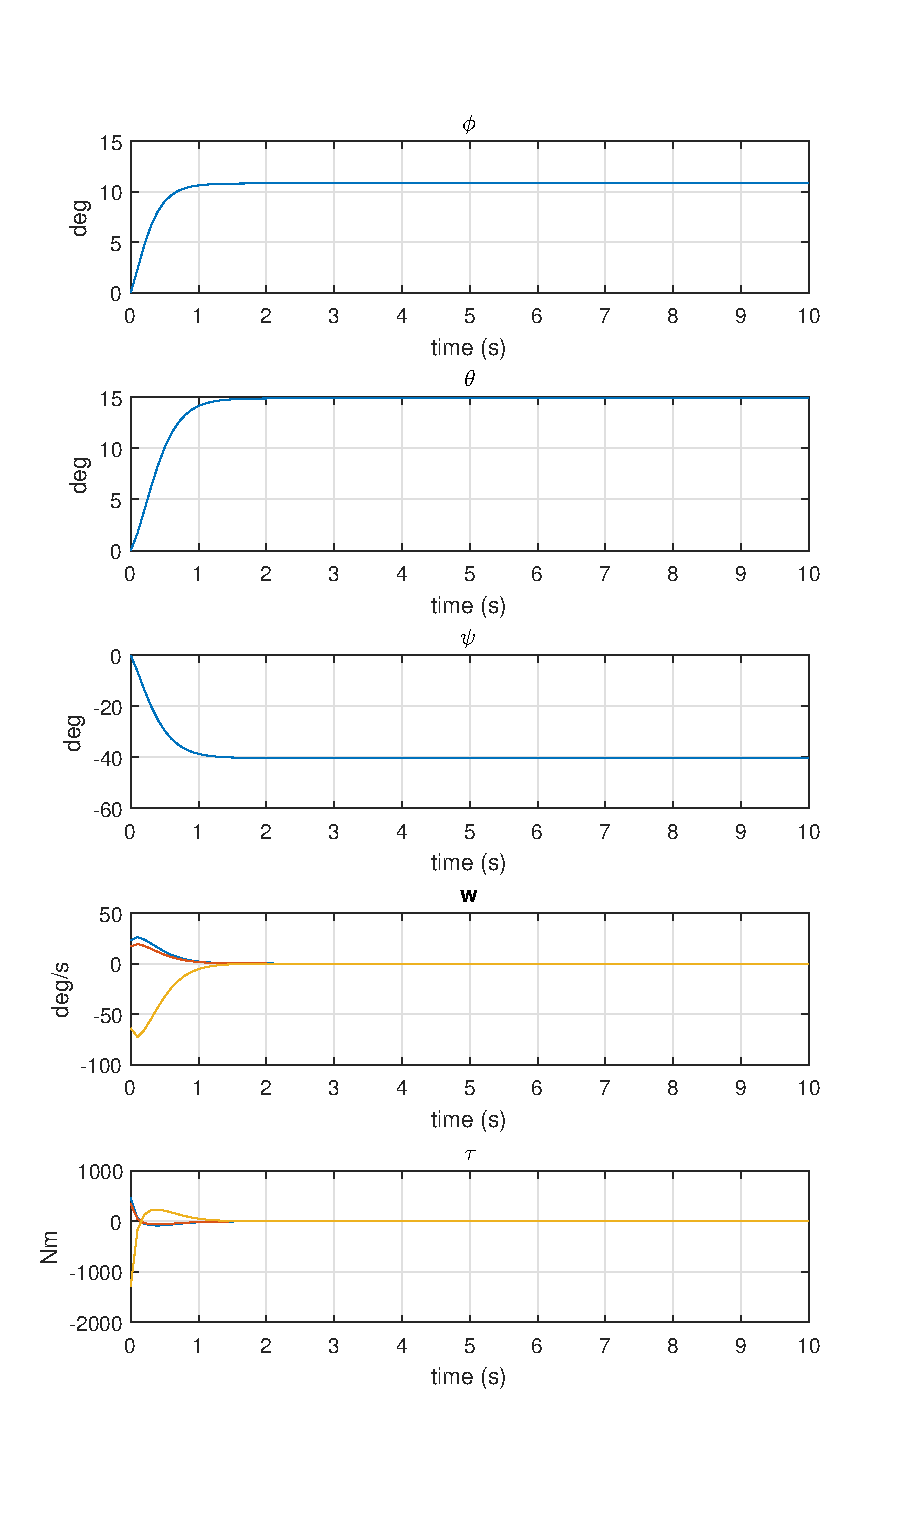
\includegraphics[width=\textwidth]{1000Rot0}
		\caption{Here is a plot where the initial angles are zero and $\boldsymbol{K}_d = \boldsymbol{K}_p=1000\boldsymbol{I}_{3\times 3}$}
		\label{fig:2a}
	\end{subfigure}
	~ %add desired spacing between images, e. g. ~, \quad, \qquad, \hfill etc. 
	%(or a blank line to force the subfigure onto a new line)
	\begin{subfigure}[b]{0.40\textwidth}
		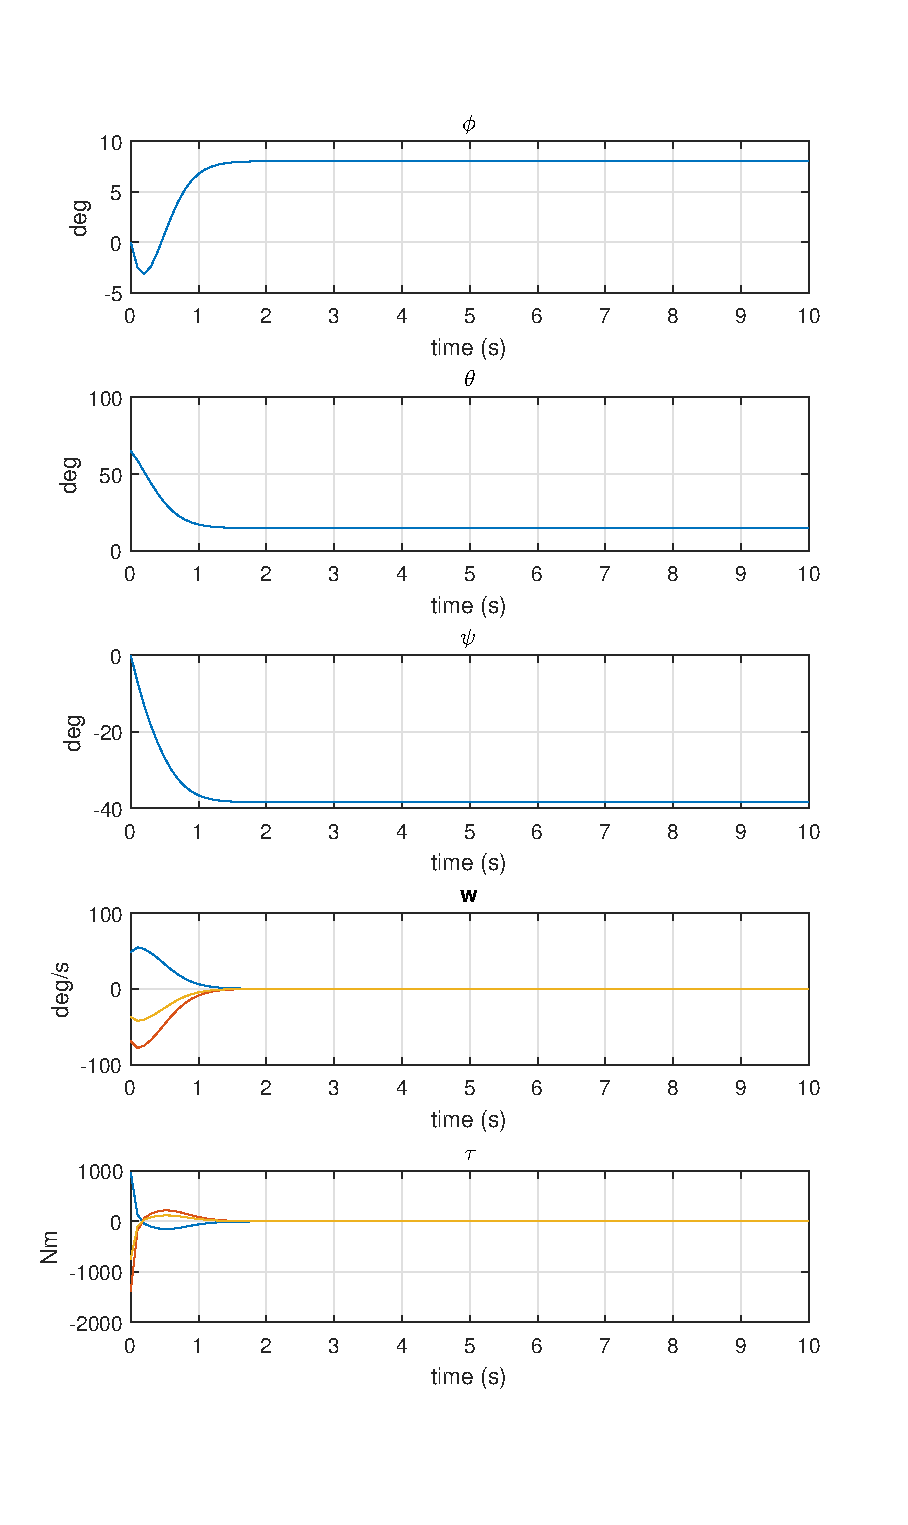
\includegraphics[width=\textwidth]{1000Rot65}
		\caption{In this plot the same $\boldsymbol{K_d}$ and $\boldsymbol{K_p}$ is used, but $\theta=65^\circ$ and the two other angles are zero}
		\label{fig:2b}
	\end{subfigure}
\end{figure}